\documentclass[10pt,a4paper]{article}\usepackage[]{graphicx}\usepackage[]{color}
%% maxwidth is the original width if it is less than linewidth
%% otherwise use linewidth (to make sure the graphics do not exceed the margin)
\makeatletter
\def\maxwidth{ %
  \ifdim\Gin@nat@width>\linewidth
    \linewidth
  \else
    \Gin@nat@width
  \fi
}
\makeatother

\definecolor{fgcolor}{rgb}{0.345, 0.345, 0.345}
\newcommand{\hlnum}[1]{\textcolor[rgb]{0.686,0.059,0.569}{#1}}%
\newcommand{\hlstr}[1]{\textcolor[rgb]{0.192,0.494,0.8}{#1}}%
\newcommand{\hlcom}[1]{\textcolor[rgb]{0.678,0.584,0.686}{\textit{#1}}}%
\newcommand{\hlopt}[1]{\textcolor[rgb]{0,0,0}{#1}}%
\newcommand{\hlstd}[1]{\textcolor[rgb]{0.345,0.345,0.345}{#1}}%
\newcommand{\hlkwa}[1]{\textcolor[rgb]{0.161,0.373,0.58}{\textbf{#1}}}%
\newcommand{\hlkwb}[1]{\textcolor[rgb]{0.69,0.353,0.396}{#1}}%
\newcommand{\hlkwc}[1]{\textcolor[rgb]{0.333,0.667,0.333}{#1}}%
\newcommand{\hlkwd}[1]{\textcolor[rgb]{0.737,0.353,0.396}{\textbf{#1}}}%

\usepackage{framed}
\makeatletter
\newenvironment{kframe}{%
 \def\at@end@of@kframe{}%
 \ifinner\ifhmode%
  \def\at@end@of@kframe{\end{minipage}}%
  \begin{minipage}{\columnwidth}%
 \fi\fi%
 \def\FrameCommand##1{\hskip\@totalleftmargin \hskip-\fboxsep
 \colorbox{shadecolor}{##1}\hskip-\fboxsep
     % There is no \\@totalrightmargin, so:
     \hskip-\linewidth \hskip-\@totalleftmargin \hskip\columnwidth}%
 \MakeFramed {\advance\hsize-\width
   \@totalleftmargin\z@ \linewidth\hsize
   \@setminipage}}%
 {\par\unskip\endMakeFramed%
 \at@end@of@kframe}
\makeatother

\definecolor{shadecolor}{rgb}{.97, .97, .97}
\definecolor{messagecolor}{rgb}{0, 0, 0}
\definecolor{warningcolor}{rgb}{1, 0, 1}
\definecolor{errorcolor}{rgb}{1, 0, 0}
\newenvironment{knitrout}{}{} % an empty environment to be redefined in TeX

\usepackage{alltt}
\usepackage[latin1]{inputenc}
\usepackage{amsmath}
\usepackage{amsfonts}
\usepackage{amssymb}
\author{Erika Martínez}
\title{Guías prácticas}
\IfFileExists{upquote.sty}{\usepackage{upquote}}{}
\begin{document}

\maketitle
\newpage

UNIDAD 3: Pr?ctica 15 - Distribuciones de probabilidad continuas.

CALCULO DE PROBABILIDADES
Ejemplo 1: 
\begin{knitrout}
\definecolor{shadecolor}{rgb}{0.969, 0.969, 0.969}\color{fgcolor}\begin{kframe}
\begin{alltt}
\hlcom{#Una persona informal hace esperar a su pareja aleatoriamente entre 0 y 90 minutos. }
\hlcom{#Harto de esta situaci?n, la persona que sufre la espera se plantea un ultim?tum; }
\hlcom{#s? al d?a siguiente su pareja tarda menos de 15 minutos mantiene la relaci?n, }
\hlcom{#s? la espera est? entre 15 y 55 minutos, decide en la siguiente cita con los }
\hlcom{#mismos criterios, mientras que si tarda m?s de 55 minutos la relaci?n termina en }
\hlcom{#ese momento. }

\hlcom{#a) Calcule la probabilidad de que la relaci?n contin?e hastala siguiente cita. }
\hlstd{x} \hlkwb{<-} \hlnum{55}\hlstd{; a}\hlkwb{=}\hlnum{0}\hlstd{; b} \hlkwb{<-} \hlnum{90}

\hlcom{#usando la funci?n propia de R }
\hlkwd{punif}\hlstd{(x,} \hlkwc{min}\hlstd{=a,} \hlkwc{max}\hlstd{=b,} \hlkwc{lower.tail}\hlstd{=}\hlnum{TRUE}\hlstd{)}
\end{alltt}
\begin{verbatim}
## [1] 0.6111111
\end{verbatim}
\begin{alltt}
\hlcom{#b) Calcule la probabilidad de que la relaci?n termine en la segunda cita.}
\hlstd{F55}\hlkwb{=}\hlkwd{punif}\hlstd{(}\hlnum{55}\hlstd{,} \hlkwc{min}\hlstd{=a,} \hlkwc{max}\hlstd{=b,} \hlkwc{lower.tail}\hlstd{=}\hlnum{TRUE}\hlstd{)}
\hlstd{F15}\hlkwb{=}\hlkwd{punif}\hlstd{(}\hlnum{15}\hlstd{,} \hlkwc{min}\hlstd{=a,} \hlkwc{max}\hlstd{=b,} \hlkwc{lower.tail}\hlstd{=}\hlnum{TRUE}\hlstd{)}
\hlstd{F55}\hlopt{-}\hlstd{F15}
\end{alltt}
\begin{verbatim}
## [1] 0.4444444
\end{verbatim}
\begin{alltt}
\hlstd{F55}\hlkwb{=}\hlkwd{punif}\hlstd{(}\hlnum{55}\hlstd{,} \hlkwc{min}\hlstd{=a,} \hlkwc{max}\hlstd{=b,} \hlkwc{lower.tail}\hlstd{=}\hlnum{TRUE}\hlstd{);F55}
\end{alltt}
\begin{verbatim}
## [1] 0.6111111
\end{verbatim}
\begin{alltt}
\hlcom{#luego multiplicando ambas probabilidades se obtiene el valor pedido 0.1728. }
\hlstd{(}\hlnum{1}\hlopt{-}\hlstd{F55)}\hlopt{*}\hlstd{( F55}\hlopt{-}\hlstd{F15)}
\end{alltt}
\begin{verbatim}
## [1] 0.1728395
\end{verbatim}
\end{kframe}
\end{knitrout}

Ejemplo 2: 
\begin{knitrout}
\definecolor{shadecolor}{rgb}{0.969, 0.969, 0.969}\color{fgcolor}\begin{kframe}
\begin{alltt}
\hlcom{#Una empresa esta buscando personal para su departamento de mercadeo. }
\hlcom{#El perfil solicitado es el de sujetos extrovertidos y creativos. }
\hlcom{#Se han presentado 50 candidatos y la empresa ha establecido como }
\hlcom{#criterio de selecci?n que los candidatos superen el percentil 80 en creatividad }
\hlcom{#y extroversi?n. Sabiendo que la variable extroversi?n (X) se distribuye seg?n una }
\hlcom{#Normal de media 5 y desviaci?n t?pica 1, que la variable creatividad (Y) }
\hlcom{#sigue una t-Student de 10 grados de libertad y que las }
\hlcom{#puntuaciones de creatividad y extroversi?n son independientes: }

\hlcom{#a) Cuantos candidatos seran seleccionados? }
\hlcom{#P(X ??? P80 ??? Y ??? P80) = P(X ??? P80) P(Y ??? P80)= (0.20)(0.20)=0.04. }
\hlcom{#Como se han presentado 50 aspirantes, ser?n seleccionadas (50) (0.04)= 2 personas. }

\hlcom{#b) ?Qu? puntuaciones debe superar un aspirante en creatividad y extroversi?n para ser admitido?}
\hlcom{#y los cuantiles-normales para la variable X: }
\hlstd{p} \hlkwb{<-} \hlkwd{c}\hlstd{(}\hlnum{0.80}\hlstd{); media}\hlkwb{=}\hlnum{5}\hlstd{; d.t}\hlkwb{=}\hlnum{1}
\hlkwd{qnorm}\hlstd{(p,} \hlkwc{mean}\hlstd{=media,} \hlkwc{sd}\hlstd{=d.t,} \hlkwc{lower.tail}\hlstd{=}\hlnum{TRUE}\hlstd{)}
\end{alltt}
\begin{verbatim}
## [1] 5.841621
\end{verbatim}
\begin{alltt}
\hlcom{#y los cuantiles-t para la variable Y: }
\hlstd{p} \hlkwb{<-} \hlkwd{c}\hlstd{(}\hlnum{0.80}\hlstd{); g.l} \hlkwb{<-} \hlnum{10}
\hlkwd{qt}\hlstd{(p,} \hlkwc{df}\hlstd{=g.l,} \hlkwc{lower.tail}\hlstd{=}\hlnum{TRUE}\hlstd{)}
\end{alltt}
\begin{verbatim}
## [1] 0.8790578
\end{verbatim}
\begin{alltt}
\hlcom{#c) Si se extraen al azar 16 candidatos, ?cu?l es la probabilidad de que su media }
\hlcom{#aritm?tica en extroversi?n sea mayor que 4.5? }
\hlcom{#Como se desea calcular P(x???4.5): }
\hlstd{n} \hlkwb{<-} \hlnum{16}\hlstd{; x} \hlkwb{<-} \hlnum{4.5}\hlstd{; mu}\hlkwb{=}\hlnum{5}\hlstd{; sigma}\hlkwb{=}\hlnum{1}\hlstd{; d.t}\hlkwb{=}\hlstd{sigma}\hlopt{/}\hlkwd{sqrt}\hlstd{(n)}
\hlkwd{pnorm}\hlstd{(x,} \hlkwc{mean}\hlstd{=mu,} \hlkwc{sd}\hlstd{=d.t,} \hlkwc{lower.tail}\hlstd{=}\hlnum{FALSE}\hlstd{)}
\end{alltt}
\begin{verbatim}
## [1] 0.9772499
\end{verbatim}
\end{kframe}
\end{knitrout}

Ejemplo 3:
\begin{knitrout}
\definecolor{shadecolor}{rgb}{0.969, 0.969, 0.969}\color{fgcolor}\begin{kframe}
\begin{alltt}
 \hlcom{#La duracion media de un modelo de marcapasos es de 7 a?os. }

\hlcom{#a) ?Cu?l es la probabilidad de que dure al menos 5 a?os? ?y menos de 3 a?os? }
\hlcom{#La probabilidad  P(x ??? 5) se obtiene as?: }
  \hlstd{x} \hlkwb{<-} \hlnum{5}\hlstd{; teta}\hlkwb{=}\hlnum{7}
\hlkwd{pexp}\hlstd{(x,} \hlkwc{rate}\hlstd{=}\hlnum{1}\hlopt{/}\hlstd{teta,} \hlkwc{lower.tail}\hlstd{=}\hlnum{FALSE}\hlstd{)}
\end{alltt}
\begin{verbatim}
## [1] 0.4895417
\end{verbatim}
\begin{alltt}
\hlcom{#De igual forma  P(X < 3): }
  \hlstd{x} \hlkwb{<-} \hlnum{3}\hlstd{; teta}\hlkwb{=}\hlnum{7}
\hlkwd{pexp}\hlstd{(x,} \hlkwc{rate}\hlstd{=}\hlnum{1}\hlopt{/}\hlstd{teta,} \hlkwc{lower.tail}\hlstd{=}\hlnum{TRUE}\hlstd{)}
\end{alltt}
\begin{verbatim}
## [1] 0.3485609
\end{verbatim}
\begin{alltt}
\hlcom{#b) Si han transcurrido ya 4 a?os desde su implantaci?n, ?cu?l es la probabilidad de que dure otros 4?}
\hlkwd{pexp}\hlstd{(}\hlnum{4}\hlstd{,} \hlkwc{rate}\hlstd{=}\hlnum{1}\hlopt{/}\hlstd{teta,} \hlkwc{lower.tail}\hlstd{=}\hlnum{FALSE}\hlstd{)}
\end{alltt}
\begin{verbatim}
## [1] 0.5647181
\end{verbatim}
\begin{alltt}
\hlcom{#c) ?Cu?nto tiempo deber?a funcionar un marcapasos para estar entre el 10% de los que m?s duran?}
\hlcom{#Hay que calcular el percentil 90: }
  \hlstd{p} \hlkwb{<-} \hlnum{0.9}\hlstd{; teta} \hlkwb{<-} \hlnum{7}
\hlkwd{qexp}\hlstd{(p,} \hlkwc{rate}\hlstd{=}\hlnum{1}\hlopt{/}\hlstd{teta,} \hlkwc{lower.tail}\hlstd{=}\hlnum{TRUE}\hlstd{)}
\end{alltt}
\begin{verbatim}
## [1] 16.1181
\end{verbatim}
\begin{alltt}
\hlcom{#d) Calcular el valor que deben tener a y b para que  P(x < a )=0.5 y  P(x > b)=0.32}
\hlkwd{qexp}\hlstd{(}\hlnum{0.5}\hlstd{,} \hlkwc{rate}\hlstd{=}\hlnum{1}\hlopt{/}\hlstd{teta,} \hlkwc{lower.tail}\hlstd{=}\hlnum{TRUE}\hlstd{)}
\end{alltt}
\begin{verbatim}
## [1] 4.85203
\end{verbatim}
\begin{alltt}
\hlcom{#y en el segundo caso, el percentil 68, b = 7.97 }
\hlkwd{qexp}\hlstd{(}\hlnum{0.68}\hlstd{,} \hlkwc{rate}\hlstd{=}\hlnum{1}\hlopt{/}\hlstd{teta,} \hlkwc{lower.tail}\hlstd{=}\hlnum{TRUE}\hlstd{)}
\end{alltt}
\begin{verbatim}
## [1] 7.97604
\end{verbatim}
\begin{alltt}
\hlcom{#o de esta otra manera }
\hlkwd{qexp}\hlstd{(}\hlnum{0.32}\hlstd{,} \hlkwc{rate}\hlstd{=}\hlnum{1}\hlopt{/}\hlstd{teta,} \hlkwc{lower.tail}\hlstd{=}\hlnum{FALSE}\hlstd{)}
\end{alltt}
\begin{verbatim}
## [1] 7.97604
\end{verbatim}
\end{kframe}
\end{knitrout}

3. GENERACION DE MUESTRAS ALEATORIAS DE LAS DISTRIBUCIONES
Ejemplo 1: 
\begin{knitrout}
\definecolor{shadecolor}{rgb}{0.969, 0.969, 0.969}\color{fgcolor}\begin{kframe}
\begin{alltt}
\hlcom{#Generar 100 n?meros aleatorios de una distribuci?n Uniforme en [-2, 4] }

\hlcom{#Definir los par?metros apropiados }
\hlstd{min} \hlkwb{<-} \hlopt{-}\hlnum{2}\hlstd{; max} \hlkwb{<-} \hlnum{4}

\hlcom{#Generar 100 n?meros aleatorios de la distribuci?n }
\hlstd{x} \hlkwb{=} \hlkwd{runif}\hlstd{(}\hlnum{100}\hlstd{, min, max); x}
\end{alltt}
\begin{verbatim}
##   [1]  3.81970921  3.42344671  0.68028756  2.85710483  0.86161155
##   [6] -0.10356160  0.94804666  0.70855223  1.51878021  0.31779432
##  [11] -1.45219109 -1.00489845 -1.23199360  0.77586313 -1.07201188
##  [16]  0.25982444 -0.16187620 -0.16476409  0.87537930  0.29263473
##  [21] -0.51793991  3.48011049 -0.02129767  1.61462834  1.06964777
##  [26] -0.26133118  1.21097333 -1.86111975  1.32378095  0.96700157
##  [31]  0.52866131 -0.74604258 -1.04556883  1.32670522  1.00409266
##  [36]  3.03478569  1.36840231  3.61482371 -0.18205365  1.94929561
##  [41] -0.56271758 -0.22513958  1.02440964  1.95226237 -1.06630512
##  [46]  0.10675079  1.34291543 -0.02636565  2.34492836  3.13116203
##  [51]  1.31330019  1.51265841 -1.20927482  3.70024679 -1.23161260
##  [56]  0.49964533  0.34865532 -1.39250274 -0.79498227  0.69057505
##  [61]  0.69550494  2.61101560  0.17691932  3.53614203 -1.29898327
##  [66]  3.29317969  2.97245616  2.90138494 -0.98595574  1.29052762
##  [71]  3.59268505 -0.55321030  3.73827497 -0.05134817 -1.59610442
##  [76]  1.76537656  2.26415426  1.20805048  3.28573639  2.79413910
##  [81]  2.09592298  0.44706239  2.80329500  1.30961489 -1.86303326
##  [86] -0.18110779  2.54330526  2.91036578 -1.78664146 -1.72212409
##  [91]  1.01878449  3.72274504  3.50832468 -1.27523900  2.62132125
##  [96]  3.21123232 -0.42331226  1.50718414  1.03912592  3.44502846
\end{verbatim}
\begin{alltt}
\hlcom{#Histograma para la nuestra aleatoria de tama?o 100 }
\hlkwd{hist}\hlstd{(x,} \hlkwc{main}\hlstd{=}\hlstr{"X ~ Uniforme(min=-2, max=4"}\hlstd{,} \hlkwc{xlab}\hlstd{=}\hlstr{"X"}\hlstd{,} \hlkwc{ylab}\hlstd{=}\hlstr{"densidad de probabilidad"}\hlstd{,}
     \hlkwc{probability}\hlstd{=}\hlnum{TRUE}\hlstd{,} \hlkwc{col}\hlstd{=}\hlstr{"green"}\hlstd{)}

\hlcom{#Graficar la funci?n de densidad, use la funci?n curve() para variable continua }
\hlkwd{curve}\hlstd{(}\hlkwd{dunif}\hlstd{(x, min, max),} \hlkwc{col}\hlstd{=}\hlstr{"blue"}\hlstd{,} \hlkwc{add}\hlstd{=}\hlnum{TRUE}\hlstd{)}
\end{alltt}
\end{kframe}
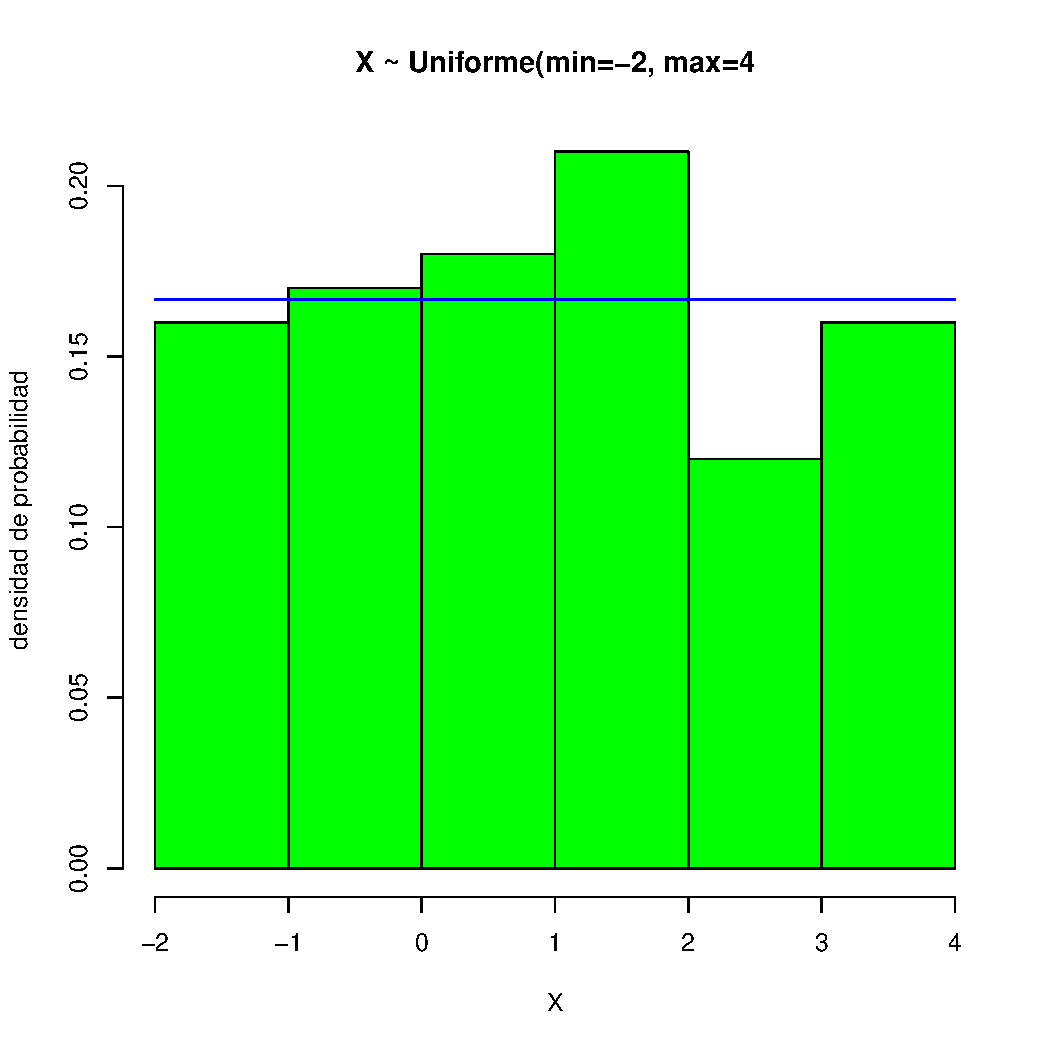
\includegraphics[width=\maxwidth]{figure/unnamed-chunk-4-1} 

\end{knitrout}

Ejemplo 2: 
\begin{knitrout}
\definecolor{shadecolor}{rgb}{0.969, 0.969, 0.969}\color{fgcolor}\begin{kframe}
\begin{alltt}
\hlcom{#Supongamos que tenemos una muestra de tama?on=200 perteneciente a una poblaci?n normal }
\hlcom{#N(10,2) con ??=10 y ??=2:}

\hlcom{#genera los valores aleatorios de la distribuci?n }
\hlstd{x.norm} \hlkwb{<-} \hlkwd{rnorm}\hlstd{(}\hlkwc{n}\hlstd{=}\hlnum{200}\hlstd{,}\hlkwc{mean}\hlstd{=}\hlnum{10}\hlstd{,} \hlkwc{sd}\hlstd{=}\hlnum{2}\hlstd{)}

\hlcom{# Podemos obtener un histograma usando la funci?n hist() }
\hlkwd{hist}\hlstd{(x.norm,} \hlkwc{breaks} \hlstd{=} \hlstr{"Sturges"}\hlstd{,} \hlkwc{freq} \hlstd{=} \hlnum{TRUE}\hlstd{,} \hlkwc{probability} \hlstd{=} \hlnum{FALSE}\hlstd{,} \hlkwc{include.lowest} \hlstd{=} \hlnum{TRUE}\hlstd{,}
\hlkwc{right}\hlstd{=} \hlnum{TRUE}\hlstd{,} \hlkwc{density} \hlstd{=} \hlkwa{NULL}\hlstd{,} \hlkwc{angle} \hlstd{=} \hlnum{45}\hlstd{,} \hlkwc{col} \hlstd{=} \hlstr{"steelblue1"}\hlstd{,} \hlkwc{border} \hlstd{=} \hlkwa{NULL}\hlstd{,}
\hlkwc{main} \hlstd{=} \hlstr{"Histograma de datos observados"}\hlstd{,} \hlkwc{axes} \hlstd{=} \hlnum{TRUE}\hlstd{,} \hlkwc{plot} \hlstd{=} \hlnum{TRUE}\hlstd{,} \hlkwc{labels} \hlstd{=} \hlnum{FALSE}\hlstd{)}
\end{alltt}
\end{kframe}
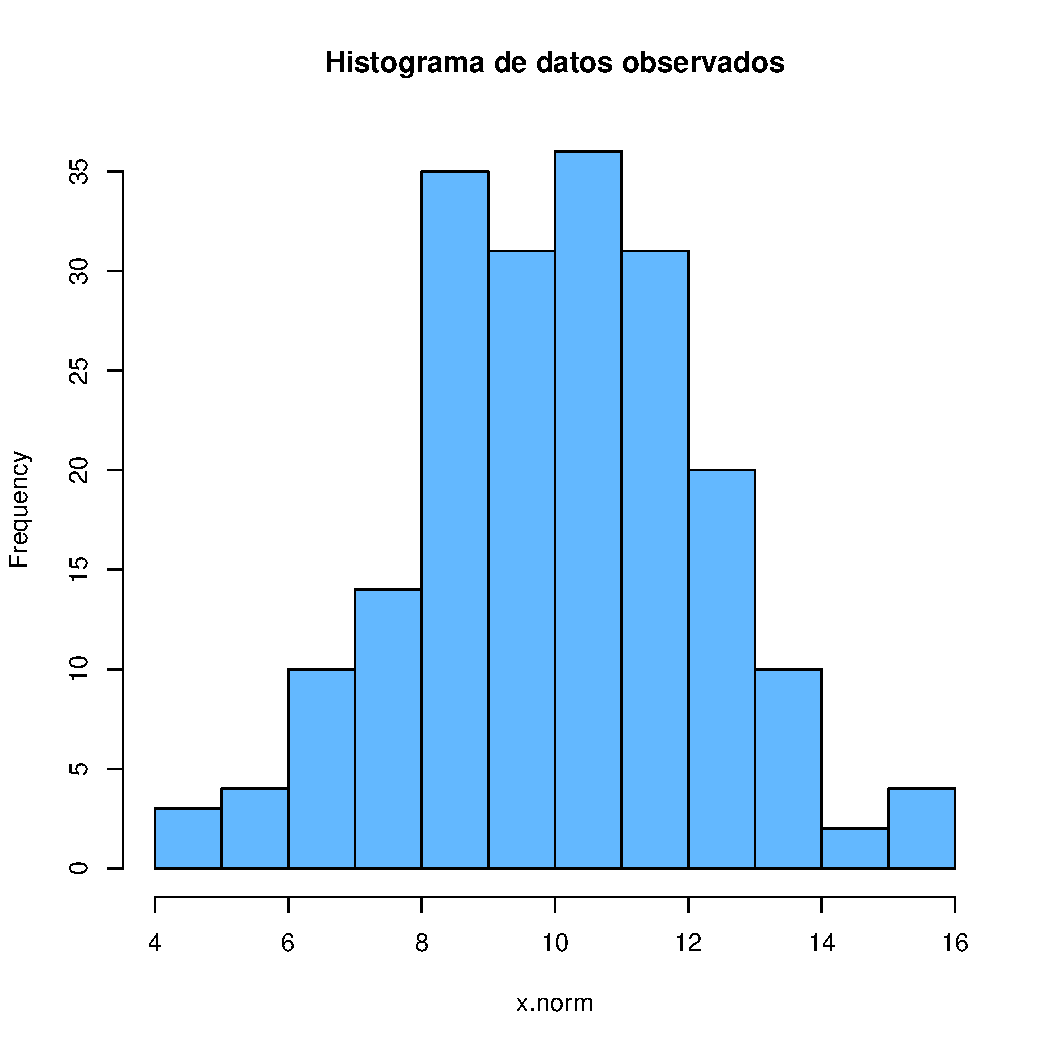
\includegraphics[width=\maxwidth]{figure/unnamed-chunk-5-1} 
\begin{kframe}\begin{alltt}
\hlcom{# Podemos estimar la densidad de frecuencia usando la funci?n density() y plot() para dibujar su gr?fica }
\hlkwd{plot}\hlstd{(}\hlkwd{density}\hlstd{(x.norm),} \hlkwc{main}\hlstd{=}\hlstr{"Densidad estimada de los datos"}\hlstd{)}
\end{alltt}
\end{kframe}
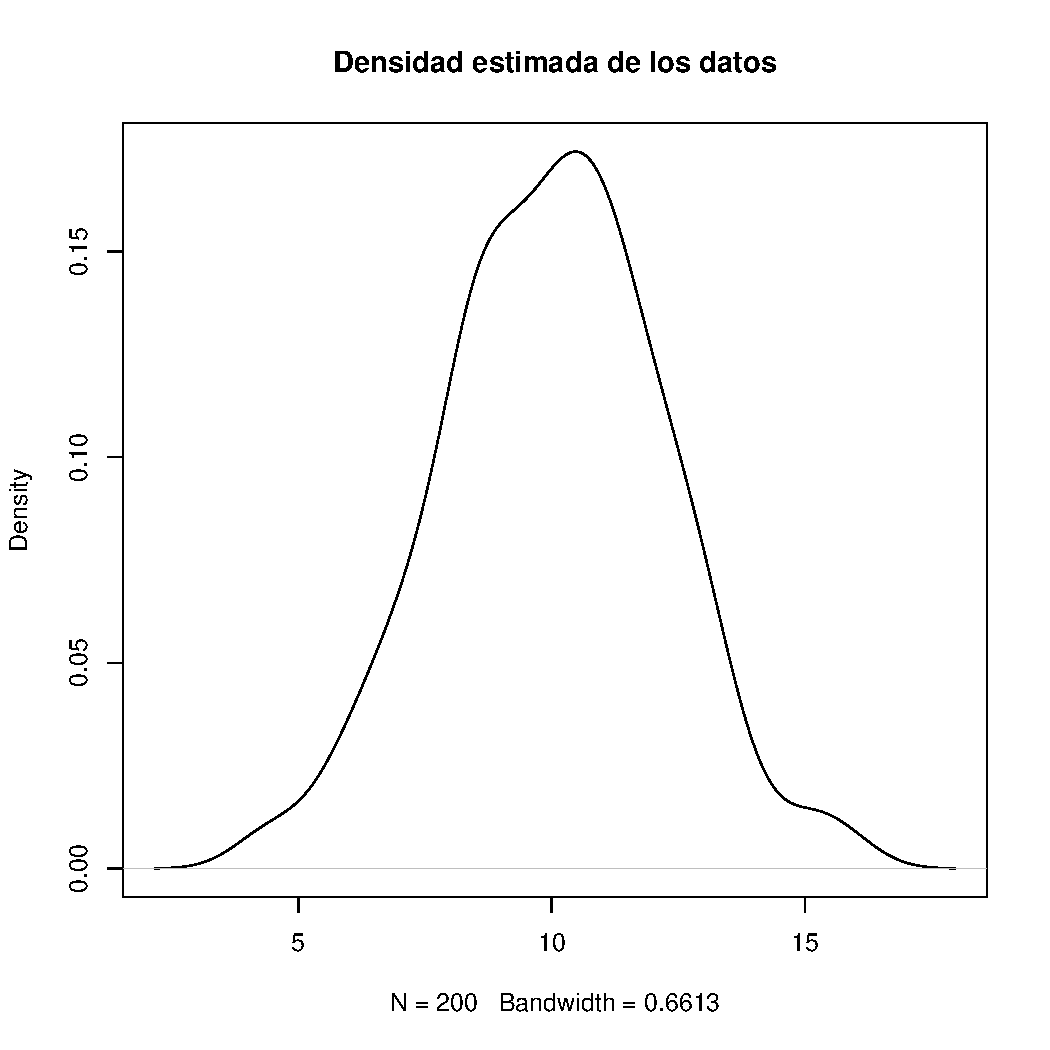
\includegraphics[width=\maxwidth]{figure/unnamed-chunk-5-2} 
\begin{kframe}\begin{alltt}
\hlcom{# R permite calcular la funci?n de distribuci?n acumulada te?rica con ecdf() }
\hlkwd{plot}\hlstd{(}\hlkwd{ecdf}\hlstd{(x.norm),}\hlkwc{main}\hlstd{=}\hlstr{"Funci?n de distribuci?n acumulada te?rica"}\hlstd{)}
\end{alltt}
\end{kframe}
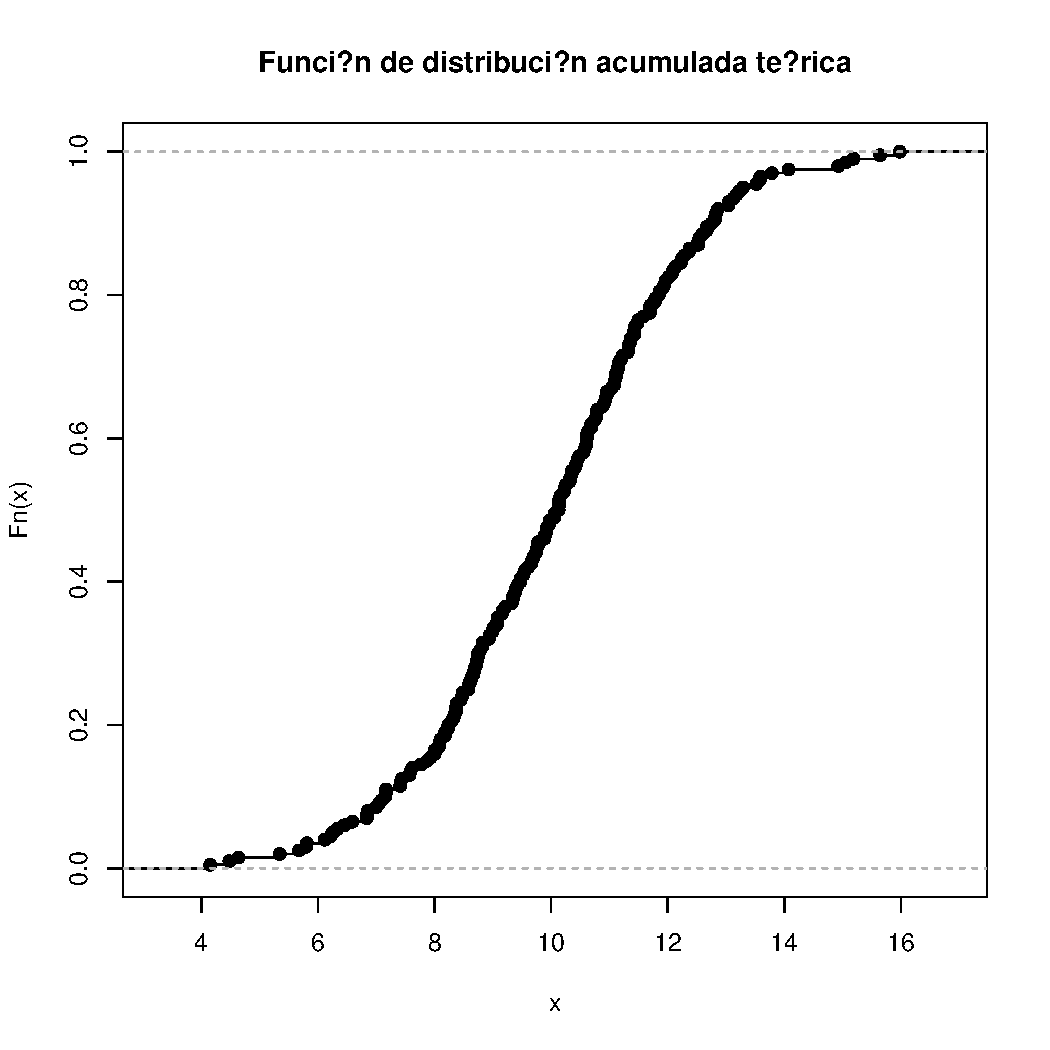
\includegraphics[width=\maxwidth]{figure/unnamed-chunk-5-3} 

\end{knitrout}

Ejemplo 3: 
\begin{knitrout}
\definecolor{shadecolor}{rgb}{0.969, 0.969, 0.969}\color{fgcolor}\begin{kframe}
\begin{alltt}
\hlcom{#Generar 100 n?meros aleatorios de una distribuci?n Normal con media 4.5 y desviaci?n est?ndar 0.75 }

\hlcom{# Definir los par?metros apropiados }
\hlstd{media} \hlkwb{<-} \hlnum{4.5}\hlstd{; desviacion} \hlkwb{<-} \hlnum{0.75}

\hlcom{# generar 100 n?meros aleatorios de la distribuci?n }
\hlstd{x} \hlkwb{=} \hlkwd{rnorm}\hlstd{(}\hlnum{100}\hlstd{, media, desviacion); x}
\end{alltt}
\begin{verbatim}
##   [1] 4.429338 4.265500 5.703503 6.915353 4.542177 3.953954 5.010443
##   [8] 4.246002 4.315193 4.711716 3.909676 4.677137 3.148630 2.965990
##  [15] 4.810213 4.077164 3.756052 4.141245 5.098877 4.487149 5.390029
##  [22] 5.080080 3.025334 3.344975 4.615169 4.060546 6.725714 4.380379
##  [29] 4.838427 5.223491 6.826793 3.428595 3.827121 4.409824 4.531692
##  [36] 5.294828 3.090587 3.710270 5.620900 4.547597 4.570558 4.112480
##  [43] 4.728451 4.141836 5.896649 4.664670 5.475036 3.132298 4.353513
##  [50] 5.515823 5.171826 5.807158 6.140113 4.788365 5.349674 3.694043
##  [57] 6.009055 4.123640 5.188616 4.384684 3.608607 4.867834 4.775455
##  [64] 5.411493 5.703831 6.130846 2.982866 4.558613 3.163125 5.039655
##  [71] 5.227904 4.740599 4.002800 3.855175 4.607228 4.816054 4.728449
##  [78] 5.666212 4.155624 3.959455 5.205610 5.884785 4.587304 4.229472
##  [85] 4.157687 4.471228 5.185206 4.829999 4.842317 4.701332 3.397415
##  [92] 4.238022 5.184821 4.800458 4.722342 4.042401 4.561183 4.706475
##  [99] 4.644746 5.908093
\end{verbatim}
\begin{alltt}
\hlcom{# Histograma para la nuestra aleatoria de tama?o 100 }
\hlkwd{hist}\hlstd{(x,}\hlkwc{main}\hlstd{=}\hlkwd{expression}\hlstd{(}\hlkwd{paste}\hlstd{(}\hlstr{"X ~ N("}\hlstd{, mu,} \hlstr{" = 4.5, "}\hlstd{, sigma,} \hlstr{" = 0.75)"}\hlstd{)),}
\hlkwc{xlab}\hlstd{=}\hlstr{"X"}\hlstd{,} \hlkwc{ylab}\hlstd{=}\hlstr{"densidad de probabilidad"}\hlstd{,} \hlkwc{probability}\hlstd{=}\hlnum{TRUE}\hlstd{,} \hlkwc{col}\hlstd{=}\hlkwd{gray}\hlstd{(}\hlnum{0.9}\hlstd{))}

\hlcom{# Graficar la funci?n de densidad te?rica, usando la funci?n curve() }
\hlkwd{curve}\hlstd{(}\hlkwd{dnorm}\hlstd{(x, media, desviacion),} \hlkwc{col}\hlstd{=}\hlstr{"red"}\hlstd{,} \hlkwc{lwd}\hlstd{=}\hlnum{2}\hlstd{,} \hlkwc{add}\hlstd{=}\hlnum{TRUE}\hlstd{)}
\end{alltt}
\end{kframe}
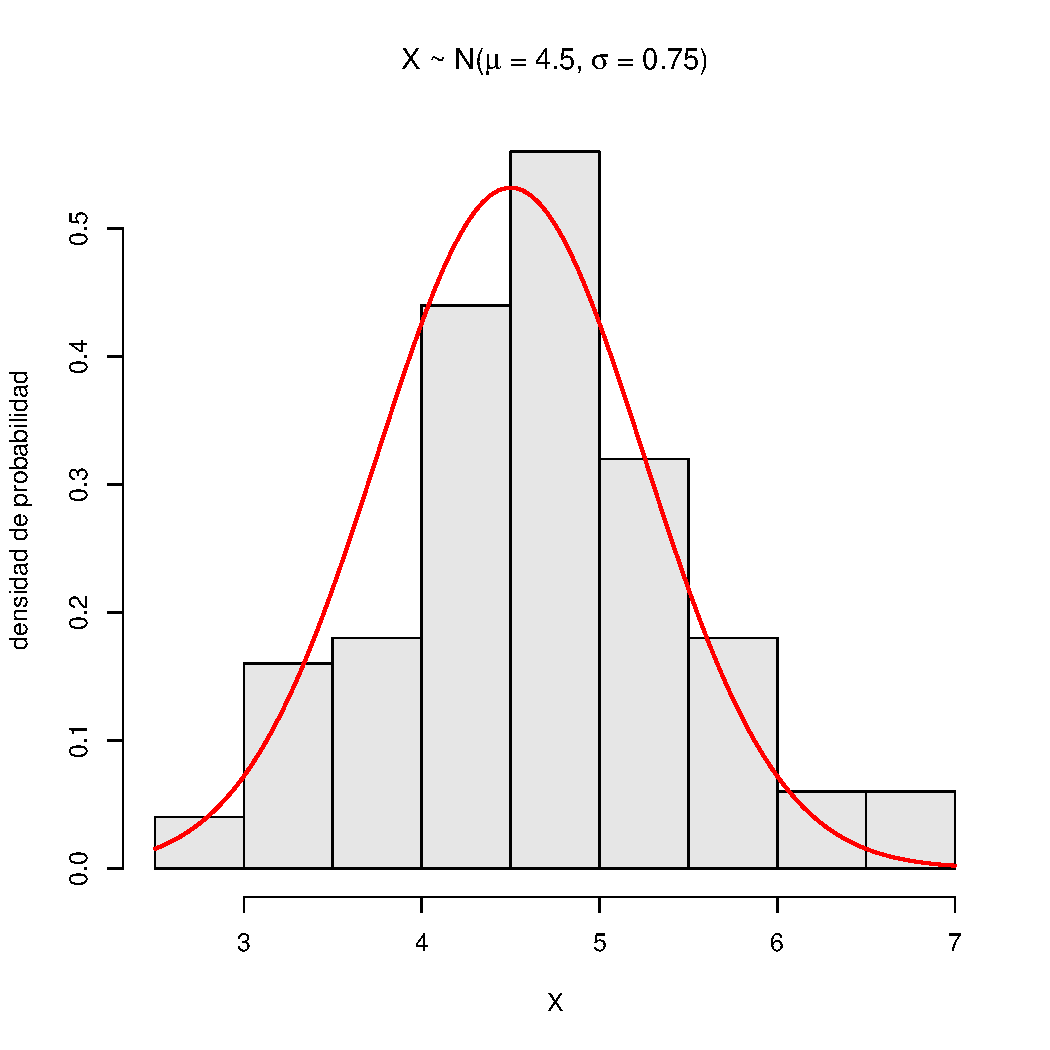
\includegraphics[width=\maxwidth]{figure/unnamed-chunk-6-1} 

\end{knitrout}

Ejemplo 4: 
\begin{knitrout}
\definecolor{shadecolor}{rgb}{0.969, 0.969, 0.969}\color{fgcolor}\begin{kframe}
\begin{alltt}
\hlcom{#Generar n?meros aleatorios de una distribuci?n exponencial. Por ejemplo, si la vida media de un }
\hlcom{#bulbo de luz es 2500 horas, uno puede pensar que el tiempo de vida es aleatorio con una distribuci?n }
\hlcom{#exponencial que tiene media 2500. El ?nico par?metro es la raz?n = 1/media.}

\hlcom{# Definir el par?metro apropiado }
\hlstd{media} \hlkwb{<-} \hlnum{2500}\hlstd{; razon} \hlkwb{<-} \hlnum{1}\hlopt{/}\hlstd{media;n}\hlkwb{=}\hlnum{100}

\hlcom{# generar 100 n?meros aleatorios de la distribuci?n }
\hlstd{x} \hlkwb{=} \hlkwd{rexp}\hlstd{(n, razon); x}
\end{alltt}
\begin{verbatim}
##   [1]  2486.630417   301.215268  5126.382760  3455.666839   426.861849
##   [6]   746.031021  2205.725843  6759.465630  3406.705444   490.953317
##  [11]  1593.325128  6322.284932  1266.337290  4176.060539  1489.167887
##  [16]  2671.999703  3314.607574 11782.773779  1697.371064   129.232030
##  [21]  1228.139448  2059.389474  3639.816858   169.053732   343.585920
##  [26]  1539.310581   149.186913  1851.334072  3770.575858  2347.165856
##  [31]  3018.558244  1713.549357  6866.956460 13765.299585  1527.245310
##  [36]  7978.475447  1706.892384  4120.193398   273.621884  1925.811728
##  [41]  4309.080853   193.666110  2079.109604   542.952684  1287.599169
##  [46]  1010.417130  4820.496712   558.549266  2319.654913  1894.919406
##  [51]  6204.069624   937.842255  5953.921326  6843.005265   649.842217
##  [56]   133.637799  4650.050406  2247.496110  6166.510447  3511.324243
##  [61]  3797.790585  1545.393717   381.456846  1579.576721  1701.857761
##  [66]   561.996764   967.008476  5271.816034   372.820594  2000.882970
##  [71]  2665.432335   325.258437   359.615904  1834.241506    36.791353
##  [76]  2087.709587  2941.752267  2033.767111   612.340065     1.369687
##  [81]  1168.955170  1708.741133   707.939303  2680.881987  1782.472350
##  [86]  4987.815255   627.729825  3723.657610  3793.557985   742.334272
##  [91]  2078.841443  1953.794332    90.696266  1853.510088  8364.158533
##  [96]  1576.392432   933.048576   854.814297   223.194397   210.448146
\end{verbatim}
\begin{alltt}
\hlcom{# Histograma para la nuestra aleatoria de tama?o 100 }
\hlkwd{hist}\hlstd{(x,} \hlkwc{main}\hlstd{=}\hlstr{"X ~ Exponencial( media = 2500 )"}\hlstd{,} \hlkwc{xlab}\hlstd{=}\hlstr{"X"}\hlstd{,}
\hlkwc{ylab}\hlstd{=}\hlstr{"densidad de probabilidad"}\hlstd{,} \hlkwc{probability}\hlstd{=}\hlnum{TRUE}\hlstd{,} \hlkwc{col}\hlstd{=}\hlstr{"purple"}\hlstd{)}

\hlcom{# Graficar la funci?n de densidad, usando la funci?n curve() }
\hlkwd{curve}\hlstd{(}\hlkwd{dexp}\hlstd{(x, razon),} \hlkwc{col}\hlstd{=}\hlstr{"blue"}\hlstd{,} \hlkwc{lwd}\hlstd{=}\hlnum{2}\hlstd{,} \hlkwc{add}\hlstd{=}\hlnum{TRUE}\hlstd{)}
\end{alltt}
\end{kframe}
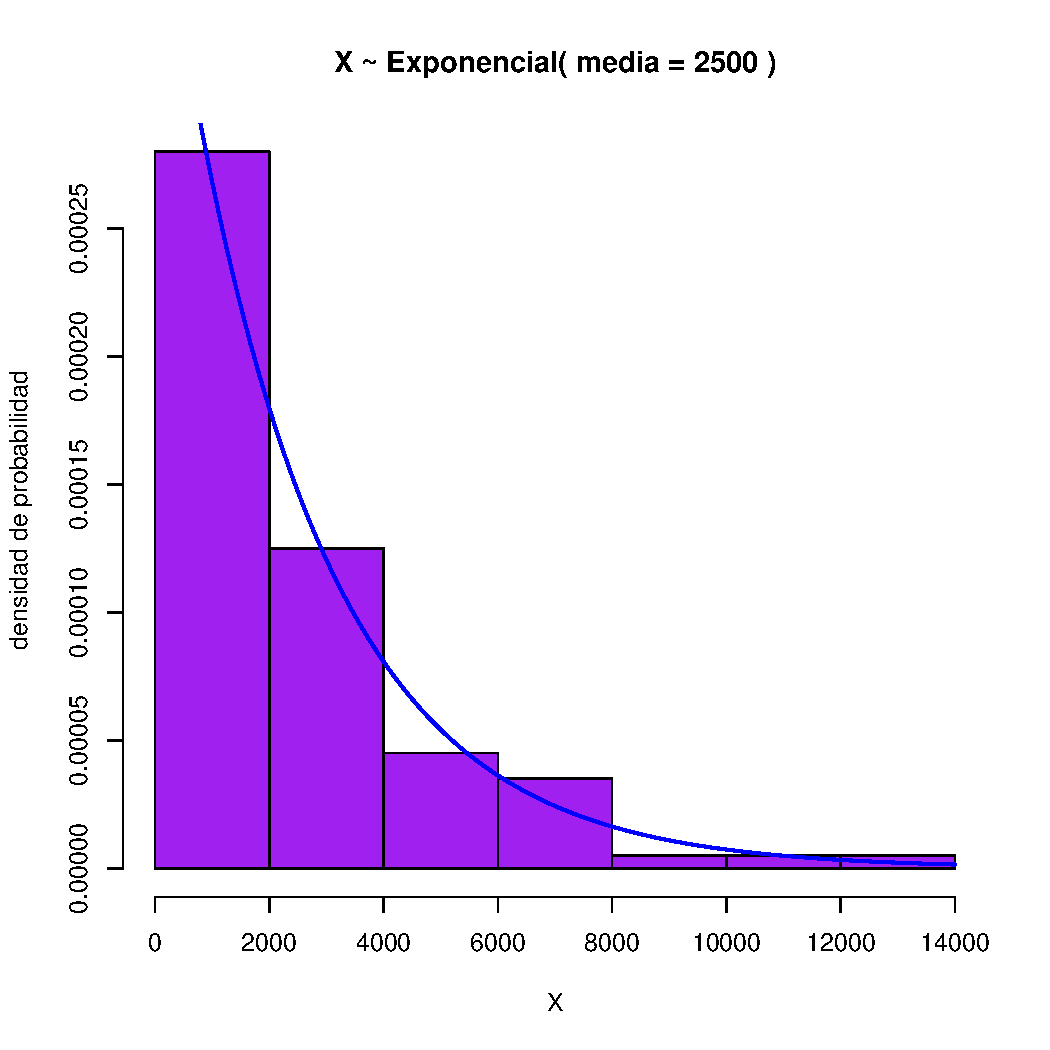
\includegraphics[width=\maxwidth]{figure/unnamed-chunk-7-1} 

\end{knitrout}

4. FUNCIONES DE DISTRIBUCION Y SU INVERSA (LOS CUANTILES).
Ejemplo 1:Para una Variable aleatoria X con distribuci?n normal de media 1 y desviacion estandar 1, cual es la probabilidad de que sea menor que 0.7? 
\begin{knitrout}
\definecolor{shadecolor}{rgb}{0.969, 0.969, 0.969}\color{fgcolor}\begin{kframe}
\begin{alltt}
\hlstd{x} \hlkwb{<-} \hlnum{0.7}
\hlstd{p} \hlkwb{<-} \hlkwd{pnorm}\hlstd{(x,} \hlkwc{mean}\hlstd{=}\hlnum{1}\hlstd{,} \hlkwc{sd}\hlstd{=}\hlnum{1}\hlstd{,} \hlkwc{lower.tail} \hlstd{=} \hlnum{TRUE}\hlstd{); p}
\end{alltt}
\begin{verbatim}
## [1] 0.3820886
\end{verbatim}
\end{kframe}
\end{knitrout}

Ejemplo 2:
\begin{knitrout}
\definecolor{shadecolor}{rgb}{0.969, 0.969, 0.969}\color{fgcolor}\begin{kframe}
\begin{alltt}
\hlcom{#Para una variable aleatoria con distribuci?n normal est?ndar, encontrar P[Z ??? 0.7 ] y P[Z> 0.7].}
\hlstd{z} \hlkwb{<-} \hlnum{0.7}
\hlstd{p1} \hlkwb{<-} \hlkwd{pnorm}\hlstd{(z,} \hlkwc{mean}\hlstd{=}\hlnum{0}\hlstd{,} \hlkwc{sd}\hlstd{=}\hlnum{1}\hlstd{); p1}
\end{alltt}
\begin{verbatim}
## [1] 0.7580363
\end{verbatim}
\begin{alltt}
\hlstd{p2} \hlkwb{<-} \hlkwd{pnorm}\hlstd{(z,} \hlkwc{mean}\hlstd{=}\hlnum{0}\hlstd{,} \hlkwc{sd}\hlstd{=}\hlnum{1}\hlstd{,} \hlkwc{lower.tail}\hlstd{=}\hlnum{FALSE}\hlstd{); p2}
\end{alltt}
\begin{verbatim}
## [1] 0.2419637
\end{verbatim}
\end{kframe}
\end{knitrout}


Ejemplo 3:
\begin{knitrout}
\definecolor{shadecolor}{rgb}{0.969, 0.969, 0.969}\color{fgcolor}\begin{kframe}
\begin{alltt}
\hlcom{#?Qu? valor de una variable aleatoria con distribuci?n normal est?ndar, tiene 75% }
\hlcom{#del ?rea a la izquierda?. }
\hlstd{p} \hlkwb{<-} \hlnum{0.75}
\hlstd{z} \hlkwb{<-} \hlkwd{qnorm}\hlstd{(p,} \hlkwc{mean}\hlstd{=}\hlnum{0}\hlstd{,} \hlkwc{sd}\hlstd{=}\hlnum{1}\hlstd{,} \hlkwc{lower.tail} \hlstd{=} \hlnum{TRUE}\hlstd{); z}
\end{alltt}
\begin{verbatim}
## [1] 0.6744898
\end{verbatim}
\end{kframe}
\end{knitrout}

Ejemplo 4:
\begin{knitrout}
\definecolor{shadecolor}{rgb}{0.969, 0.969, 0.969}\color{fgcolor}\begin{kframe}
\begin{alltt}
\hlcom{#?Cu?l es la probabilidad a la derecha de 18.55 para una Variable aleatoria X con }
\hlcom{#distribuci?n Chi-cuadrado de 12 grados de libertad? }
\hlstd{x} \hlkwb{<-} \hlnum{18.55}\hlstd{; gl} \hlkwb{<-} \hlnum{12}
\hlstd{p} \hlkwb{<-} \hlkwd{pchisq}\hlstd{(x, gl,} \hlkwc{lower.tail} \hlstd{=} \hlnum{FALSE}\hlstd{); p}
\end{alltt}
\begin{verbatim}
## [1] 0.09998251
\end{verbatim}
\end{kframe}
\end{knitrout}

\end{document}
